\documentclass{article}
\usepackage[top=1cm, left=1.5cm, right=1.5cm, bottom=1.5cm]{geometry}
\usepackage{graphicx}
\usepackage{wrapfig}
\graphicspath{{./img/}}
\usepackage{amsmath}
\usepackage{tcolorbox}
\usepackage{tikz-cd}
\usepackage{amssymb}
\setlength{\parindent}{0pt}
\setlength{\parskip}{1em} 

\title{Ecuaciones Lineales}
\date{28/11/2023}
\author{Pablo DS} 

\begin{document}
\maketitle
\section{Sistemas Lineales}

En matemáticas la palabra “lineal” tiene un significado muy amplio. Una gran parte de la teoría de álgebra lineal elemental es, de hecho, una generalización de las propiedades de la línea recta.

\begin{tcolorbox}[colback=green!20!white,colframe=green!80!black,title=Propiedades de la Recta]
    \begin{itemize}
        \item[-] La \textbf{pendiente} $m$ de una recta que pasa por los puntos $(x_1, y_1)$ y $(x_2, y_2)$ está dada por $$m=\frac{y_2-y_1}{x_2-x_1} = \frac{\Delta y}{\Delta x} \quad si \quad x_1 \neq x_2$$
        \item[-] Si $x_2 - x_1 = 0$ y $y2 \neq y1$, entonces la recta es vertical y se dice que la pendiente es indefinida.
        \item[-] Cualquier recta (a excepción de aquella que tiene una pendiente indefinida) se puede describir con su ecuación en la forma pendiente-ordenada al origen $\mathbf{y= mx + b}$, donde $m$ es la pendiente de la recta y $b$ es la ordenada al origen
        \item[-] Dos rectas distintas son paralelas si y sólo si tienen la misma pendiente. 
        \item[-] Las rectas paralelas al eje $x$ tienen pendiente cero
        \item[-] Las rectas paralelas al eje y tienen pendiente indefinida.
    \end{itemize}

\end{tcolorbox}

Una ecuación lineal en las variables $ x_1,x_2,\dots, x_n $ es una ecuación que puede escribirse de la forma $ a_1x_1,a_2x_2,\dots, a_nx_n=b$ donde $b$ y los coeficientes $a_1,a_2,\dots, a_n$ son números reales o complejos, el subíndice n puede ser cualquier número entero positivo. En los problemas de la vida real, $n$ puede ser 50 o 5000, o incluso mayor. Aquí se utiliza la palabra lineal porque la gráfica de la ecuación es una linea recta.

En muchas apliciones se nos da $b$ y a las constantes $ a_1,a_2,\dots, a_n $ donde debemos determinar los números $ x_1,x_2,\dots, x_n $ denominados \textbf{incógnitas}, que satisfacen la ecuación.

Una \textbf{solución} de una ecuación lineal es una sucesión $ n $ de números $ s_1,s_2,\dots, s_n $ que tienen la propiedad de satisfacer a la ecuación, cuando los valores $(s_1, s_2, \dots, s_n)$ se sustituyen por $(x_1, x_2, \dots, x_n)$ en la ecuación.

Un \textbf{sistema de $m$ ecuaciones lineales con $n$ incógnitas $ x_1,x_2,\dots, x_n $}, (al que podemos llamar sistema lineal) es un conjunto de $m$ ecuaciones lineales, cada una con $ n $ incógnitas; el cual se puede denotar como:

\begin{equation}
    \begin{matrix}
        \begin{aligned}
            a_{11}x_1 + a_{12}x_2 + \dots + a_{1n}x_n = b_1\\
            a_{21}x_1 + a_{22}x_2 + \dots + a_{2n}x_n = b_2\\
            \vdots \phantom{aaaaaaaa} \vdots \phantom{aaaaaaaaaa} \vdots \phantom{aaaaaa} \vdots\\
            a_{m1}x_1 + a_{m2}x_2 + \dots + a_{mn}x_n = b_m\\
        \end{aligned}
    \end{matrix}
\end{equation}

\pagebreak

Una solución del sistema es una lista $s_1, s_2, \dots, s_n$ de números que hace que cada ecuación sea una afirmación verdadera cuando los valores $(s_1, s_2, \dots, s_n)$ se sustituyen por $(x_1, x_2, \dots, x_n)$, respectivamente. El conjunto de todas las soluciones posibles se denomina conjunto de soluciones del sistema lineal. Dos sistemas lineales se denominan equivalentes si tienen el mismo conjunto de soluciones. Las preguntas que surgen son: ¿tiene este sistema varias soluciones y, de ser así, cuántas? 

Encontrar el conjunto solución de un sistema de dos ecuaciones lineales en dos variables es fácil porque cada ecuación corresponde a una línea recta, por lo cual la solución equivale a encontrar la intersección de dos rectas. Dos rectas no tienen por qué intersecarse en un único punto; si no son paralelas, entonces se intersectan en un punto, por el contrario, si son paralelas entonces o no se intersectan o son la misma recta y se intersectan en infinitos puntos.

La gráfica de cada ecuacion de un sistema de $2 \times 2$ es una línea recta, que denotamos mediante $l_1$ y $l_2$, respectivamente. Si $x = s1$, $y = s2$ es una solución del sistema lineal, entonces el punto (s1, s2) pertenece a ambas rectas, $l_1$ y $l_2$. De manera recíproca, si el punto (s1, s2) está en ambas rectas, $l_1$ y $l_2$, entonces $x = s1$, $y = s2$ es una solución para el sistema lineal.

\begin{tcolorbox}[colback=blue!10!white,colframe=blue!60!black,title=Posibles casos]
    \begin{itemize}
        \item[1.] El sistema tiene una solución única; esto es, las rectas $l_1$ y $l_2$ se intersecan exactamente en un punto.
        \item[2.] El sistema no tiene solución; es decir, las rectas $l_1$ y $l_2$ no se intersecan.
        \item[3.] El sistema tiene un número infinito de soluciones; en otras palabras, las rectas $l_1$ y $l_2$ coinciden.
    \end{itemize}
\end{tcolorbox}

Se dice que un sistema es inconsistente si no tiene solución y que un sistema es consistente si tiene 1 solución o infinitas soluciones.

\begin{figure}[ht]
  \centerline{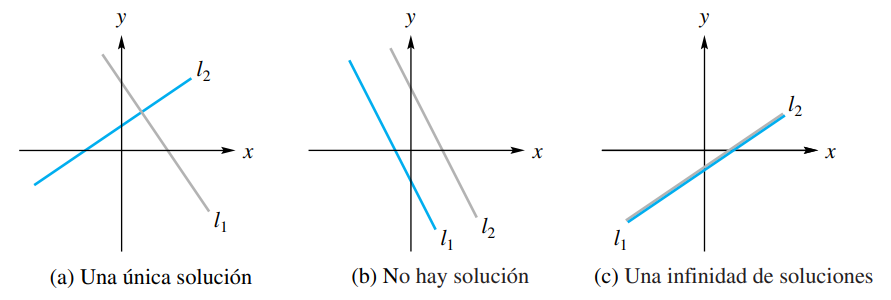
\includegraphics[width=0.7\textwidth]{image5.png}}
  \caption{Ilustración de casos con 2 incógnitas}
  \label{}
\end{figure}

Ahora, consideremos un sistema lineal de tres ecuaciones con tres incógnitas, $x, y$ y $z$:

$$\begin{matrix}
    a_1x + b_1y + c_1z =d_1\\ 
    a_2x + b_2y + c_2z =d_2\\ 
    a_3x + b_3y + c_3z =d_3
\end{matrix}$$

La gráfica de cada una de estas ecuaciones es un plano, y se denota con $P_1, P_2$ y $P_3$ respectivamente. Como en el caso de un sistema lineal de dos ecuaciones con dos incógnitas, el sistema lineal puede tener una solución única, no tener solución o tener una infinidad de soluciones. Estos 3 casos se extrapolan a sistemas de ecuaciones de $m \times n$.

\begin{figure}[ht]
  \centerline{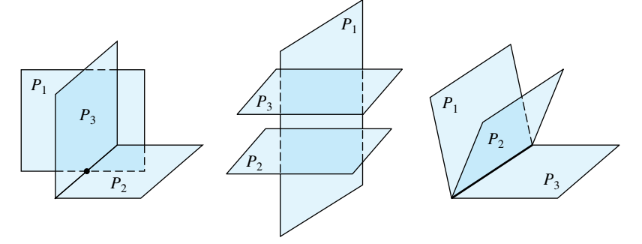
\includegraphics[width=0.6\textwidth]{image4.png}}
  \caption{Ilustración de casos con 3 incógnitas}
  \label{}
\end{figure}

\subsection{Resolviendo Sistemas de Ecuaciones}

Para resolver las siguientes ecuaciones lineales usaremos el método de elminación, el cuál consiste en eliminar variable(s) de alguna ecuación hasta aislar una sola para obtener su valor y después sustituir ese valor en las demás ecuaciones; para ello se hará uso de las operaciones elementales por filas, las cuales el efectuarlas no afecta el sistema de ecuaciones. 

\begin{tcolorbox}[colback=blue!10!white,colframe=blue!60!black,title=Operaciones Elementales por filas]
    \begin{itemize}
        \item[1.] Intercambiar dos ecuaciones o dos filas.
        \item[2.] Multiplicar una ecuación por una constante diferente de cero.
        \item[3.] Multiplicar una ecuación y sumarla a otra.
    \end{itemize}
\end{tcolorbox}

\begin{large}
    Ejemplo 1
\end{large}
Considere el sistema lineal

\begin{equation*}
    \begin{aligned}
            x &- 3y = -7\\
            2x &-6y = \phantom{-} 7
    \end{aligned}
\end{equation*}

Decidimos eliminar x. Para ello sumamos (-2) veces la primera ecuación a la segunda y obtenemos:

\begin{equation*}
    \begin{aligned}
            x & - 3y = -7\\
            0x & +0y = 21
    \end{aligned}
\end{equation*}

Cuya segunda ecuación no tiene sentido. Esto significa que la solución del sistema lineal es el conjunto vacío o bien el sistema no tiene solución.

\begin{large}
    Ejemplo 2
\end{large}
Considere el sistema lineal

\begin{equation*}
    \begin{aligned}
            x & +2y -3z = -4\\
            2x & +\phantom{2}y -3z = \phantom{-} 4
    \end{aligned}
\end{equation*}

Para eliminar $x$, sumamos (-2) veces la primera ecuación a la segunda y obtenemos

\begin{equation*}
    \begin{aligned}
            x & +2y &-3z = -4\\
            & -3y &+3z = 12
    \end{aligned}
\end{equation*}

Despejamos $y$ en la segunda ecuación para obtener $$y=z-4$$ donde $z$ puede ser cualquier numero real. Entonces, con base en la primera ecuación obtenemos 

\begin{equation*}
    \begin{matrix}
            x + 2y - 3z = -4\\
            x = -4 -2y +3z\\
            x= z + 4
    \end{matrix}
\end{equation*}

Por lo tanto, una solución para el sistema lineal es: 

\begin{equation*}
    \begin{aligned}
            x & = r + 4\\
            y & = r - 4\\
            z &= r
    \end{aligned}
\end{equation*}

Donde $r$ es cualquier número real. Esto significa que el sistema linea tiene un número infinito de soluciones. Cada vez que asignamos un valor a $r$,obtenemos otra solución.

\begin{large}
    \textbf{Ejemplo 3}
\end{large}
Considere el sistema lineal

\begin{equation*}
    \begin{aligned}
            x & +2y + 3z = 6\\
            2x & -3y + 2z = 14\\
            3x & +y - z = -2
    \end{aligned}
\end{equation*}

Para eliminar $x$, sumamos (-2) veces la primera ecuación a la segunda y (-3) veces la primera ecuación a la tercera, lo que da por resultado

\begin{equation*}
    \begin{aligned}
            x & +2y + 3z = 6\\
            & -7y - 4z = 2\\
            & -5y -10z = -20
    \end{aligned}
\end{equation*}

Después eliminamos $y$, por lo que multiplicamos la tercera ecuación por $-\frac{1}{5}$ para obtener

\begin{equation*}
    \begin{aligned}
            x & +2y & + 3z &= 6\\
            & -7y & - 4z &= 2\\
            &\phantom{-98} y & + 2z &= 4
    \end{aligned}
\end{equation*}

Intercambiamos la segunda y tercer ecuación

\begin{equation*}
    \begin{aligned}
            x & +2y & + 3z &= 6\\
            &\phantom{-98} y & + 2z &= 4\\
            & -7y & - 4z &= 2\\
    \end{aligned}
\end{equation*}

Ahora sumamos 7 veces la segunda ecuación a la tercera, para obtener

\begin{equation*}
    \begin{aligned}
            x & +2y & + 3z &= 6\\
            &\phantom{-98} y & + 2z &= 4\\
            & & 10z &= 30\\
    \end{aligned}
\end{equation*}

Por lo que $z=3$ y sustituyendo este valor en la segunda ecuación encontramos que $y=-2$. Al sustituir estos valores en la primera ecuación, finalmente obtenemos $x=1$ 

\subsection{Gauss-Jordan}

Antes de resolver otros sistemas de ecuaciones es conveniente introducir una notación que simplifica la escritura de cada paso del procedimiento mediante el concepto de matriz.

\begin{tcolorbox}[colback=blue!10!white,colframe=blue!60!black,title=Definición]
    Una matriz A de $m \times n$ es un arreglo rectangular de $mn$ números reales (o complejos) ordenados en m filas horizontales y n columnas verticales
\end{tcolorbox}

\begin{large}
    \textbf{Matriz de Coeficientes}
\end{large}

Es aquella matriz que únicamente contiene los coeficientes de las incógnitas.

\begin{equation*}
    \begin{matrix}
        \begin{array}{rrrr}
            2x_1 & 4x_2 & 6x_3 &=18\\
            4x_1 & 5x_2 & 6x_3 &=24\\
            3x_1 & x_2  & -2x_3 &=4            
        \end{array}
    \end{matrix}
    \quad \quad A = \begin{pmatrix}
        \begin{array}{rrr}
            2 & 4 & 6 \\
            4 & 5 & 6 \\
            3 & 1 & -2         
        \end{array}    
    \end{pmatrix}
\end{equation*}

\begin{large}
    \textbf{Matriz Aumentada}
\end{large}

Es aquella matriz que representa un sistema de ecuaciones lineales, donde la línea vertical separa la parte de los coeficientes (a la izquierda) de la parte de los términos independientes (a la derecha).

\begin{equation*}
    \begin{matrix}
        \begin{array}{rrrr}
            2x_1 & 4x_2 & 6x_3 &=18\\
            4x_1 & 5x_2 & 6x_3 &=24\\
            3x_1 & x_2  & -2x_3 &=4            
        \end{array}
    \end{matrix}
    \quad \quad A = \left(\begin{array}{rrr|r}
        2 & 4 & 6 & 18\\
        4 & 5 & 6 & 24\\
        3 & 1 & -2& 4
    \end{array}\right)
\end{equation*}

También se puede escribir como $Ax = b$, donde 

\begin{alignat*}{2}
    x= \begin{pmatrix}
        x_1\\
        x_2\\
        \vdots\\
        x_n
    \end{pmatrix} 
& \hspace{ 4em}%
\quad y \quad b = 
    \begin{pmatrix}
        b_1\\
        b_2\\
        \vdots\\
        b_m
    \end{pmatrix} 
\end{alignat*}

Se ha visto que multiplicar una ecuación por un número diferente de cero da por resultado una nueva ecuación equivalente, si se suma un múltiplo de una ecuación a otra del sistema se obtiene otra ecuación equivalente y por último, si se intercambian dos ecuaciones en un sistema de ecuaciones se obtiene un sistema equivalente. Como se vió anteriormente estas son las operaciones elementales por filas. El proceso de aplicar las operaciones elementales por filas para simplificar una matriz aumentada se llama reducción por filas. 

El primer número diferente de cero en una fila (si lo hay) se llama \textbf{entrada principal para esa fila}. 

Una matriz se encuentra en forma escalonada si cumple con las siguientes propiedades:

\begin{tcolorbox}[colback=blue!10!white,colframe=blue!60!black,title=Propiedades de la Forma Escalonada]
    \begin{itemize}
        \item[-] Todas las filas cuyos elementos son todos cero aparecen en la parte inferior de la matriz.
        \item[-] La entrada principal en cualquier fila está a la derecha de la entrada principal de la fila anterior
        \item[] Todas las entradas en una columna por debajo de un pivote son ceros.
    \end{itemize}   
    Una matriz se encuentra en la \textbf{forma escalonada reducida por filas} si se cumplen las siguientes condiciones:
    \begin{itemize}
        \item[-] La entrada principal en cualquier fila es 1.
        \item[-] La entrada principal es el único elemento distinto de 0 en su columna.
    \end{itemize}    
\end{tcolorbox}

\begin{large}
    \textbf{Ejemplo Forma Escalonada}
\end{large}

Las entradas principales (.) pueden tener cualquier valor diferente de 0; las otras entradas (*) pueden tener cualquier valor (incluyendo cero).

\begin{alignat*}{2}
    \begin{pmatrix}
        .&*&*&*\\
        0&.&*&*\\
        0&0&0&0\\
        0&0&0&0
    \end{pmatrix}
    & \hspace{ 4em}%
    \begin{pmatrix}
        0&.&*&*&*&*&*&*&*&*\\
        0&0&0&.&*&*&*&*&*&*\\
        0&0&0&0&.&*&*&*&*&*\\
        0&0&0&0&0&.&*&*&*&*\\
        0&0&0&0&0&0&0&0&.&*
    \end{pmatrix}
\end{alignat*}

\begin{tcolorbox}[colback=green!20!white,colframe=green!80!black,title=Pivote]
    Un pivote en una matriz es el primer componenete diferente de cero en una fila de una matriz.
\end{tcolorbox}

\begin{large}
    \textbf{Ejemplo Forma Escalonada Reducida}
\end{large}

Los pivotes son 1 y los demás elementos en su columna son 0.

\begin{alignat*}{2}
    \begin{pmatrix}
        1&0&*&*\\
        0&1&*&*\\
        0&0&0&0\\
        0&0&0&0
    \end{pmatrix}
    & \hspace{ 4em}%
    \begin{pmatrix}
        0&1&*&0&0&0&*&*&0&*\\
        0&0&0&1&0&0&*&*&0&*\\
        0&0&0&0&1&0&*&*&0&*\\
        0&0&0&0&0&1&*&*&0&*\\
        0&0&0&0&0&0&0&0&1&*
    \end{pmatrix}
\end{alignat*}

Cualquier matriz distinta de cero puede reducirse en más de una matriz en forma escalonada, utilizando diferentes secuencias de operaciones de fila. Sin embargo, la forma escalonada reducida que se obtiene de una matriz es única.

\begin{tcolorbox}[colback=green!20!white,colframe=green!80!black,title=Unicidad de la Forma Escalonada Reducida]
    Cada matriz es equivalente en fila a una y sólo una matriz escalonada reducida.
\end{tcolorbox}

\begin{large}
    Ejemplo Forma Escalonada por renglones
\end{large}

\begin{equation*}
    \begin{pmatrix}
        \begin{array}{rrr|r}
            2 & 4 & 6 & 18\\
            4 & 5 & 6 & 24\\
            3 & 1 & -2 & 4
        \end{array}
    \end{pmatrix}
    \xrightarrow{\stackrel{R_1 \rightarrow \frac{1}{2}R_1}{}}
    \begin{pmatrix}
        \begin{array}{rrr|r}
            1 & 2 & 3 & 9\\
            4 & 5 & 6 & 24\\
            3 & 1 & -2 & 4
        \end{array}
    \end{pmatrix}
\end{equation*}

\begin{equation*}
    \xrightarrow{\overset{\begin{aligned} R_2 \rightarrow R_2 - 4R_1 \\ R_3 \rightarrow R_3 - 3R_1\end{aligned}}{}} 
    \begin{pmatrix}
        \begin{array}{rrr|r}
            1& 2 & 3 & 9\\
            0 &-3 &-6 &-12 \\
            0&-5 &-11 &-23
        \end{array}
    \end{pmatrix}
    \xrightarrow{\stackrel{R_2 \rightarrow \frac{1}{3}R_2}{}}
    \begin{pmatrix}
        \begin{array}{rrr|r}
            1 & 2 & 3 & 9\\
            0 & 1 & 2 & 4\\
            0 & 5 &-11&-23
        \end{array}
    \end{pmatrix}
\end{equation*}

Ya casi tenemos la matriz escalonada, solo tenemos que hacer cero el valor de la segunda incóginita de la tercer ecuación

\begin{equation*}
    \xrightarrow{\overset{R_3 \rightarrow R_3 + 5R_2}{}} 
    \begin{pmatrix}
        \begin{array}{rrr|r}
            1 & 2 & 3 & 9\\
            0 & 1 & 2 & 4 \\
            0 & 0 &-1 &-3
        \end{array}
    \end{pmatrix}
\end{equation*}

\begin{large}
    Sustitución Hacia Atrás
\end{large}

La matriz aumentada del sistema se encuentran ahora en la forma escalonada por renglones y se puede ver de inmediato que $x_3 = 3$. Después se usa la sustitución hacia atrás para despejar primero$x_2$ y después $x_1$. La segunda ecuación queda $x_2 + 2x_3 = 4$. Entonces $x_2 + 2(3) = 4$ y $x_2 =-2$. De igual manera, de la primera ecuación se obtiene $x_1 + 2(-2) + 3(3) = 9$  con lo que se obtiene que $x1 = 4$. Así, de nuevo se obtiene la solución $(4, -2, 3)$. El método de solución que se acaba de emplear se llama \textbf{eliminación gaussiana}.

\begin{tcolorbox}[colback=blue!10!white,colframe=blue!60!black,title=Métodos]
    \begin{large}
        \textbf{Eliminación de Gauss Jordan}
    \end{large}

    Se reduce por fila la matriz aumentada a la forma escalonada reducida por filas usando el método de eliminación. Si en algún momento hay un cero en la diagonal principal, se intercambian filas para eliminar el cero de la diagonal principal. \newline

    \begin{large}
        \textbf{Eliminación Gaussiana}
    \end{large}

    Se reduce por renglón la matriz aumentada a la forma escalonada por filas, se despeja el valor de la última incógnita y después se usa la sustitución hacia atrás para las demás incógnitas.
\end{tcolorbox}

La eliminación de Gauss-Jordan es el proceso de resolución de un sistema de ecuaciones mediante la reducción por renglones de la matriz aumentada a la forma escalonada reducida por renglones.

La eliminación gaussiana es el proceso de resolver un sistema de ecuaciones al reducir por renglones la matriz aumentada a la forma escalonada por renglones y utilizando la sustitución hacia atrás.

Al resolver sistemas de ecuaciones en una computadora se
prefiere el método de eliminación gaussiana porque significa menos operaciones elementales por filas, aunque a veces es esencial obtener la forma escalonada reducida por renglones de una matriz, en estos casos la eliminación de Gauss-Jordan es el método preferido.

\begin{large}
    \textbf{Solución de un sistema de 2 ecuaciones con 4 incógnitas}
\end{large}

\begin{equation*}
    \begin{aligned}
    x_1 &+ 3x_2 &- 5x_3 &+ x_4 &= 4 \\
    2x_1 &+ 5x_2 &- 2x_3 &+ 4x_4 &= 6    
    \end{aligned}
\end{equation*}

\begin{equation*}
    \begin{pmatrix}
        \begin{array}{rrrr|r}
            1 & 3 & -5 & 1 & 4\\
            2 & 5 & -2 & 4 & 6
        \end{array}
    \end{pmatrix}
\xrightarrow{\stackrel{R_2 \rightarrow R_2 - 2R_1}{}}
    \begin{pmatrix}
        \begin{array}{rrrr|r}
            1 & 3 & -5 & 1 & 4\\
            0 & -1 & 8 & 2 & -2
        \end{array}
    \end{pmatrix}
\end{equation*}

\begin{equation*}
    \xrightarrow{\stackrel{R_2 \rightarrow -R_2}{}}
    \begin{pmatrix}
        \begin{array}{rrrr|r}
            1 & 3 & -5 & 1 & 4\\
            0 & 1 & -8 & -2 & 2
        \end{array}
    \end{pmatrix}
\xrightarrow{\stackrel{R_1 \rightarrow R_1 - 3R_2}{}}
    \begin{pmatrix}
        \begin{array}{rrrr|r}
            1 & 0 & 19 & 7 & -2\\
            0 & 1 & -8 & -2 & 2
        \end{array}
    \end{pmatrix}
\end{equation*}

La matriz de coeficiente se encuentra en forma escalonada y reducida por renglones. Es evidente que existe un número infinito de soluciones. Los valores de las variables $x_3$ y $x_4$ se pueden escoger de manera arbitraria. Entonces $$x_2 = 2 + 8x_3 + 2x_4$$ $$x_1 = -2 -19x_3 -7x_4$$ Por lo tanto, todas las soluciones se representan por $$(-2 -19x_3 -7x_4, 2 + 8x_3 + 2x_4, x_3, x_4)$$ Por ejemplo, si $x3 = 1$ y $x_4 = 2$ se obtiene la solución $(235, 14, 1, 2)$.

\begin{tcolorbox}[colback=green!20!white,colframe=green!80!black,title=Soluciones en un Sistema con más Incógnitas que Ecuaciones]
    Cuando se tienen más incógnitas que ecuaciones en un sistema lineal, o no se tiene solución (inconsistente) o tiene infinitas soluciones (indeterminado).

    Es importante destacar que la presencia de soluciones infinitas no implica necesariamente que todas las combinaciones de valores sean válidas. Pueden existir restricciones adicionales que limiten las soluciones aceptables.
\end{tcolorbox}

\begin{large}
    \textbf{Problema de Pesca}
\end{large}

Un departamento de pesca y caza del estado proporciona tres tipos de comida a un lago que alberga a tres especies de peces. Cada pez de la especie 1 consume cada semana un promedio de 1 unidad del alimento A, 1 unidad del alimento B y 2 unidades del alimento C. Cada pez de la especie 2 consume cada semana un promedio de 3 unidades del alimento A, 4 del B y 5 del C. Para un pez de la especie 3, el promedio semanal de consumo es de 2 unidades del alimento A, 1 unidad del alimento B y 5 unidades del C. Cada semana se proporcionan al lago 25 000 unidades del alimento A, 20 000 unidades del alimento B y 55 000 del C. Si suponemos que los peces se comen todo el alimento, ¿cuántos peces de cada especie pueden coexistir en el lago? Sean x1, x2 y x3 el número de peces de cada especie que hay en el ambiente del lago.

\begin{equation*}
    \begin{aligned}
        x_1 &+ 3x_2 &+ 2x_3 &= 25,000\\
        x_1 &+ 4x_2 &+ x_3 &= 20,000\\
        2x_1 &+ 5x_2 &+ 5x_3 &= 55,000
    \end{aligned}
\end{equation*}

La matriz aumentada del sistema es:

\begin{equation*}
    \begin{pmatrix}
        \begin{array}{rrr|r}
            1 & 3 & 2 & 25,000\\
            1 & 4 & 1 & 20,000 \\
            2 & 5 & 5 & 55,000
        \end{array}
    \end{pmatrix}
\end{equation*}

Utilizando reducción de Gauss-Jordan

\begin{equation*}
    \xrightarrow{\overset{\begin{aligned} R_2 \rightarrow R_2 - R_1 \\ R_3 \rightarrow R_3 - 2R_1\end{aligned}}{}} 
    \begin{pmatrix}
        \begin{array}{rrr|r}
            1& 3 & 2 & 25,000\\
            0 & 1 &-1 &-5,000 \\
            0 & -1 & 1 & 5,000
        \end{array}
    \end{pmatrix}
    \xrightarrow{\overset{\begin{aligned} R_1 \rightarrow R_1 - 3R_2 \\ R_3 \rightarrow R_3 + R_2\end{aligned}}{}} 
    \begin{pmatrix}
        \begin{array}{rrr|r}
            1 & 0 & 5 & 40,000\\
            0 & 1 & -1 & -5,000\\
            0 & 0 & 0 & 0
        \end{array}
    \end{pmatrix}
\end{equation*}

Por consiguiente, se tiene un número infinito de soluciones dada por: 

\begin{equation*}
    \begin{aligned}
        x_1 = 40,000 - 5x_3\\
        x_2 = x_3 - 5,000\\
        x_3 = \mathbb{Z}^+
    \end{aligned}
\end{equation*}

Por supuesto, como se vio anteriormente, que un sistema tenga infinitas soluciones no significa que todas las soluciones sean válidas. En este caso los valores que pueden tomar las incógnitas deben ser enteros, pues no se puede tener por ejemplo 5.6 peces; además se debe tener $x_1 \geq 0, x_2 \geq 0$ y $x_3 \geq 0$. Como $x_2 = x_3 - 5,000 \geq 0$, se tiene $x_3 \geq 5,000$. Esto significa que $0 \leq x_1 \leq 40,000 - 5(5,000)= 15,000$. Por último, como $40,000 - 5x_3 \geq 0$, se tiene que $x3 \leq 8,000$. Esto significa que las poblaciones que pueden convivir en el lago con todo el alimento consumido son: 

\begin{equation*}
    \begin{aligned}
        x_1 = 40,000 -5x_3\\
        x_2 = x_3 - 5,000\\
        5,000 \leq x_3 \leq 8,000
    \end{aligned}
\end{equation*}

\end{document}